\chapter{Introduction}


\section{Background}
A part of computer graphics is to create non-photorealistic images. A method to do this is to stylize 3D scenes. Stylizing an object means creating an image that imitates the style of an artist who would have drawn it on a sheet of paper. There exist many different styles like hand drawing, brush painting, pointillism painting, stippling, watercolor painting, etc. The two main methods to stylize is to use textures mapped on the objects of the scene or to use marks/splats which are 2d images.

\section{Problem Statement}


The main problem of stylizing a 3D object in an animation is \textit{temporal coherence}. The \textit{temporal coherence} problem in non-photorealistic rendering encompasses both spatial and temporal aspects of the marks. The effect given by the stylization has to be kept if the object is moving, rotating and scaling. Many research has been done to solve this problem of \textit{temporal coherence} \cite{vergne_implicit_2011, benard_dynamic_2009, bleron_motion-coherent_2018}. Bénard et al. separate this problem is three sections inspired by previous work\cite{meier_painterly_1996, cunzi_dynamic_nodate, breslav_dynamic_nodate, benard_state---art_2011} but they show that an ideal solution (Figure \ref{problem_temporal_coherence} a)  does not exists. Even \textit{Loving Vincent} \cite{LovingVincent} that was done by artists frame by frame has problems of marks popping because they cannot follow perfectly the flow motion of a scene. Neglect one of these three goals provide artifacts (Figure \ref{problem_temporal_coherence} b-d).

\begin{figure}[H]
    \begin{center}
    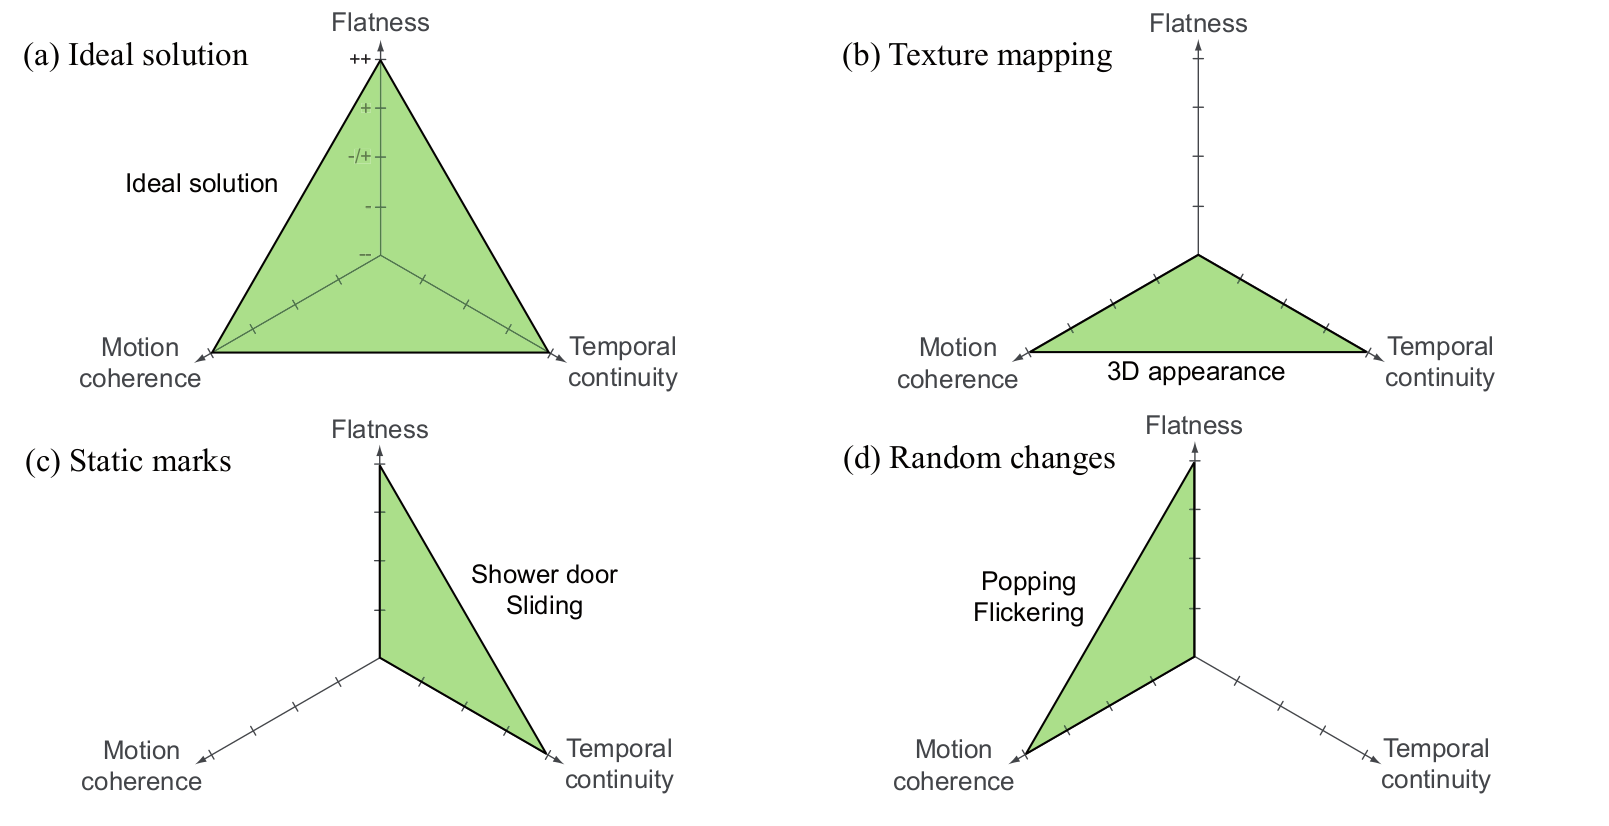
\includegraphics[scale=0.3]{pics/temporal_coherence.png}
    \end{center}
    \caption{Problem involve by temporal coherence depending of the flatness, temporal continuity, motion coherence.}
    \label{problem_temporal_coherence}
\end{figure}

\subsection{Flatness}

The impression of drawing on a flat surface gives the \textit{flatness}. The stylization has a good \textit{flatness} if the image rendered has a good 2D appearance. In order to keep this effect, the size and the distribution of the marks of your stylization have to be independent of the distance between the stylized object and the camera.

\subsection{Motion Coherence}

\textit{Motion coherence} is a correlation between the motion of marks and the motion of the 3D object. Bad \textit{Motion coherence} will give the impression to see the scene through a semi-transparent layer of marks, this is called \textit{shower door} effect \cite{meier_painterly_1996}, an example to illustrate what happens when there is a bad \textit{Motion coherence} is the movie \textit{Loving Vincent}\cite{LovingVincent}. The goal is to provide in 2D screen space a perceptual impression of motion as
close as possible to the 3D displacement in object space.

\subsection{Temporal continuity}

\textit{Temporal continuity} is the quality of minimizing changes from frame to frame to ensure fluid animations. In order to have good \textit{temporal continuity}, the marks of the image have to fade slowly during the animation. Human perception is very sensitive to \textit{temporal incoherence} according to some perceptual studies\cite{percept_studies, Schwarz_2009}. \newline


The problem introduced in the works of Bénard et al.\cite{benard_state---art_2011} is the difficulty to have a ideal solution, the one that has a good \textit{flatness}, a good \textit{motion coherence} and a good \textit{temporal continuity}. These three goals are inherently contradictory when you improve one you neglect one or maybe more. So researchers work to find solutions that make \textit{trade-offs} between these three goals. We built our approach trying to take the better of each different approach, looking at what works well and what can be integrated into our method.

\section{Contents of this report}

After an analysis of the previous works on stylizing scene, we searched on how we could have a solution that permits to control the 3 axes of the \textit{temporal coherence}. We defined what were the advantages of each method of stylizing: marks-based method and texture-based method. The texture-based method has a very good \textit{temporal continuity} and \textit{motion coherence} at a price of bad \textit{flatness} and a poor variety of style. On the over hand, the mark-based method has good flatness and a wide variety of possibles styles but introducing a problem of anchoring these marks. From this analysis, we decided to use marks to stylize our object but we had to find a way to anchor these splat. We used the good property of the textures mapped in object space. They permit to have a perfect \textit{temporal continuity} and \textit{motion coherence} so we used the textures to anchor our marks to the object but we did not ordinary texture to do so, we used procedural textures because we can manipulate them easily and are cheap to render. \newline

This is our solution, draw marks anchored to the object thanks to procedural textures in an image. We implemented this solution in OpenGL in order to render all images with the power of the GPU. In the figure \ref{some_results} you can see some results done with our method.

\begin{figure}[H]
    \begin{center}
    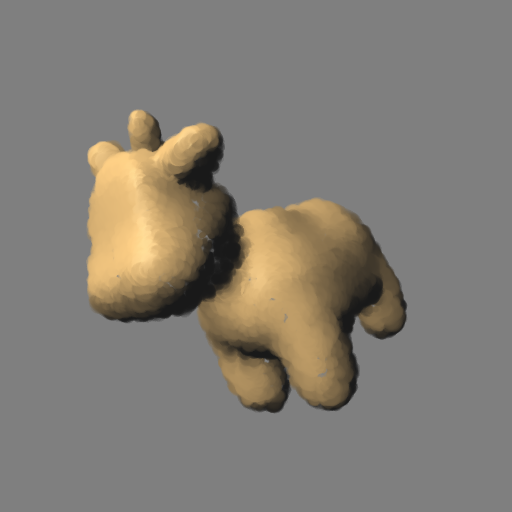
\includegraphics[width=50mm, height=50mm]{Resultats/spotPoint/final.png}
    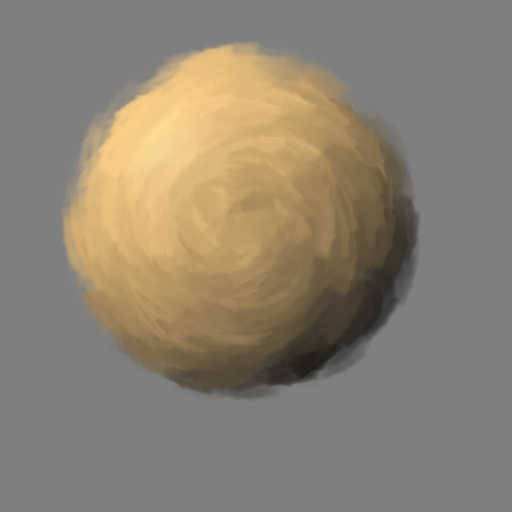
\includegraphics[width=50mm, height=50mm]{Resultats/painting1/final.png}
    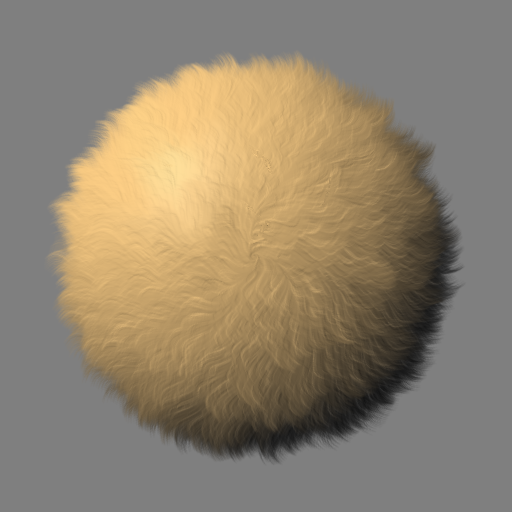
\includegraphics[width=50mm, height=50mm]{Resultats/bouledepoil1/final.png}
    \end{center}
    \caption{Some results of stylizing with our method of procedural stylization (left: pointillism rendering, middle: brush painting, right: hair rendering).}
    \label{some_results}
\end{figure}
